\chapter{Opis projektnog zadatka}
		
		
		Cilj ovog projekta jest stvoriti web aplikaciju kojom korisnik može lakše upravljati kućnim otpadom. Razvrstavanje i odlaganje različitih vrsta otpada postalo je zahtjevno pa bi aplikacija olakšala taj posao informiranjem koja vrsta otpada pripada kojem odlagalištu. Osim toga, aplikacija nudi mogućnost slanja zahtjeva za odvoz glomaznog otpada i slanja zahtjeva za resurse prikupljanja otpada. U slučaju da su građani nezadovoljni uslugom zbrinjavanja otpada, postoji mogućnost slanja pritužbi. Ovakva aplikacija odlično je rješenje za automatizaciju cijelog procesa zbrinjavanja otpada.
		
		Trenutačno postoji web aplikacija Čistoće \url{https://www.cistoca.hr/} koja informira građane gdje bi mogli odložiti otpad i u kojim terminima te se na tu adresu mogu slati zahtjevi za odvoz glomaznog otpada.\\
		\begin{figure}[H]
			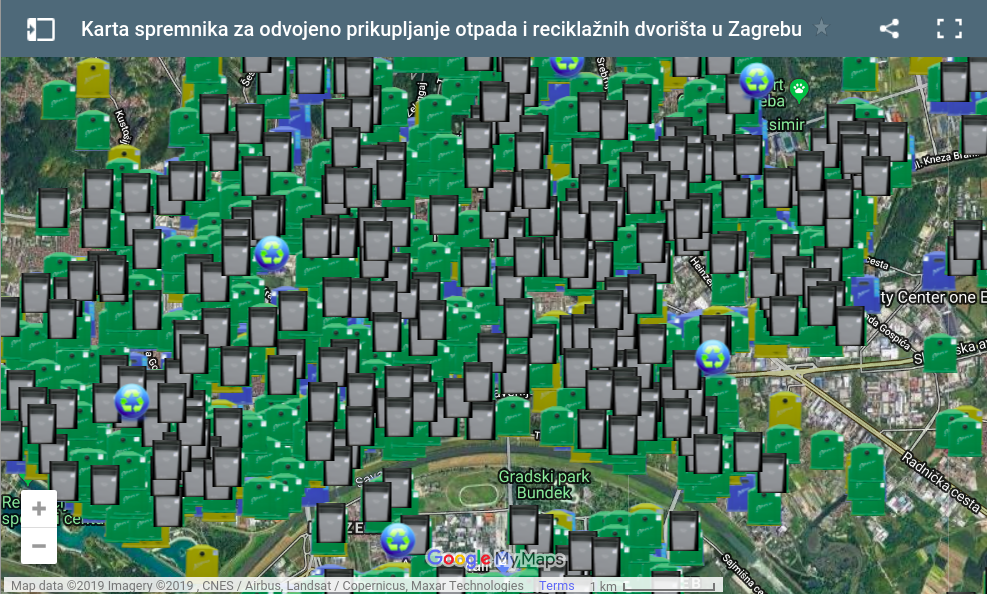
\includegraphics[width=\linewidth]{slike/karta.png}
			\centering
			\caption{Karta odlagališta na stranici \url{https://www.cistoca.hr/}}
			\label{fig:karta}
		\end{figure}
		\begin{figure}[H]
			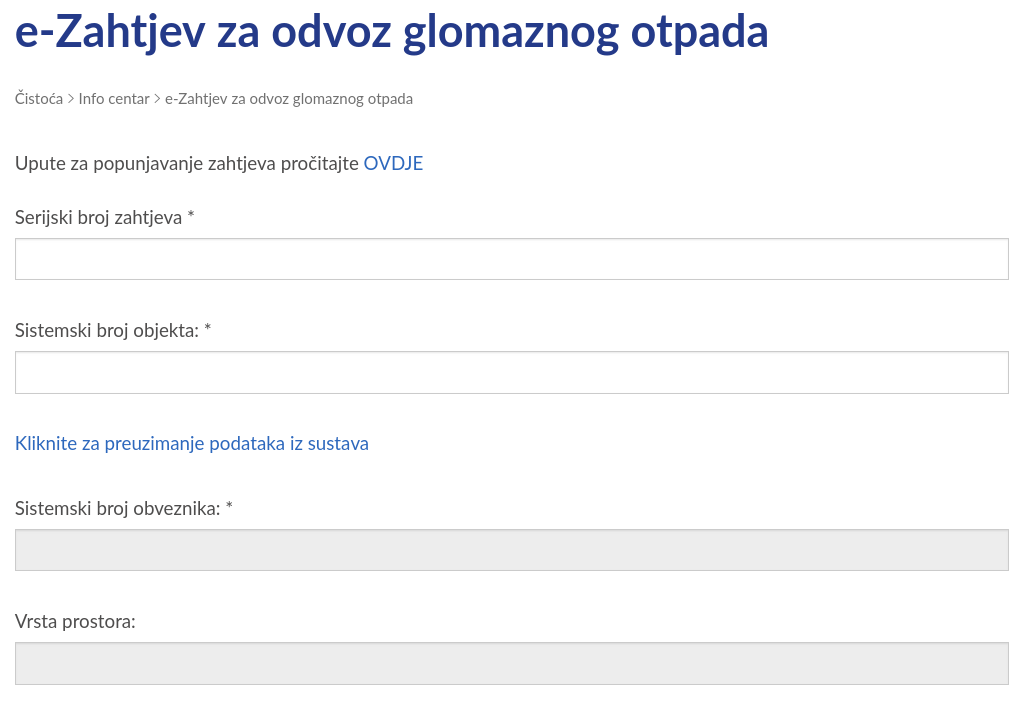
\includegraphics[scale=0.4]{slike/zahtjevi.png}
			\centering
			\caption{Slanje zahtjeva za odvoz glomaznog otpada s \url{https://www.cistoca.hr}}
			\label{fig:zahtjev}
		\end{figure}
		
		
		
		Ipak, postoji potreba za novom aplikacijom jer trenutačna nedovoljno informira o razvrstavanju otpada te se ne može izravno poslati pritužba Čistoći. Prednosti nove aplikacije su i dobra preglednost te jednostavnost njezina korištenja.\\
		
		Aplikaciju smiju koristiti registrirani građani (dalje: građani), zaposlenici poduzeća koje zbrinjava otpad (dalje: zaposlenici) i administratori. Građanima treba omogućiti registraciju, pri čemu je potrebno navesti:
		
		\begin{packed_item}
			\item \text{ime}
			\item \text{prezime}
			\item \text{adresu stanovanja (ulica, broj i mjesto)}
			\item \text{adresu e-pošte }
			\item \text{korisničko ime}
			\item \text{lozinku}
		\end{packed_item}
		
		\noindent Zaposlenici se registriraju tako što navode:
		
		\begin{packed_item}
			\item \text{korisničko ime}
			\item \text{lozinku}
		\end{packed_item}
	
		\noindent{Administratori se evidentiraju izravno u bazi podataka.}\\\\
		
		Glavni zadatak aplikacije je informiranje građana oko svega što je vezano uz upravljanje kućnim otpadom. Podatke za informiranje građana ažuriraju zaposlenici i administratori te će biti dostupni svim registriranim građanima. Osim toga, aplikacija treba omogućiti slanje zahtjeva građana za dodatnim resursima za prikupljanje kućnog otpada, zahtjeva za odvozom krupnog otpada i slanje pritužbi.\\\\
		
		\noindent Informiranje građana uključuje sljedeće funkcionalnosti:
		
		\begin{packed_enum}
			\item odabir naziva ili kategorije proizvoda koji se razvrstava, za koje se navodi tip resursa za dozvoljeno odlaganje (određeni tip vrećice, tip kante ili kontejnera, uz grafički prikaz)
			\item dostupnost odlagališta otpada u blizini mjesta stanovanja, uz otvaranje Google Mapsa s odgovarajućim lokacijama i opisom tih lokacija (vrste podržanog otpada, radno vrijeme)
			\item informacije o terminima odvoza kućnog otpada za određenu lokaciju
			\item informacije o poduzeću koje zbrinjava otpad (uključujući kontakt-informacije)
		\end{packed_enum}
		\text{}
	
		\noindent{Informacije će biti specifične za grad  u kojem se zbrinjava otpad te će administrator unositi te informacije i zaposlenici će moći mijenjati neke informacije.}\\
		
		Prilikom slanja zahtjeva građani na aplikaciji moraju imati preglednik vrsta resursa i upis komada odabranog resursa za odlaganje, uz navedeno obrazloženje. Slanje pritužbi treba uključivati detaljni opis pritužbe. Nakon slanja pritužbe ili zahtjeva, potrebno je omogućiti ispis svih poslanih informacija u PDF-formatu i iskrcavanje PDF-a na lokalno računalo. Osim funkcionalnosti printanja zahtjeva i pritužbi, građani će moći vidjeti povijest odgovora na svoje zahtjeve i pritužbe koje su im poslali zaposlenici.\\
		
		\noindent Osim građana postoje još dvije vrste korisnika, a to su:
		
		\begin{packed_item}
			\item \text{zaposlenik}
			\item \text{administrator}
		\end{packed_item}
		\text{}\\
		Zadaća zaposlenika:
		
		\begin{packed_item}
			\item pregledavanje zahtjeva i pritužbi građana te odgovaranje na upite
			\item mijenjanje informacija
		\end{packed_item}
	
		  Zaposlenicima će biti prikazan popis zahtjeva i pritužbi poredan po vremenu kako bi na njih lakše odgovarali. Nakon što se jednom odgovori na pritužbu ili zahtjev, ta pritužba ili zahtjev više neće biti prikazana korisniku.\\
		  
        \noindent Zadaća administratora:
        
        \begin{packed_item}
        	\item smiju mijenjati sve informacije
        	\item brisanje bilo kojeg korisničkog računa
        \end{packed_item}
		
		
		Aplikacija bi se mogla unaprijediti pregledom računa za odvoz smeća te prikazom stanja duga. 
		Pod informacije bi se mogli staviti cjenik usluga zbrinjavanja otpada i materijali za informiranje građana zbog čega je važno razvrstavati otpad. Još jedna ideja bi bila dodavanje slanja zahtjeva za čišćenje privatnih površina.
		
		\eject